

We now present the compound loss designed for training PU-GAN in an end-to-end fashion.

%In this subsection, we illustrate loss functions that are employed to train our PU-GAN in an end-to-end fashion, which consists of an \emph{adversarial loss}, a \emph{uniform loss} and a \emph{reconstruction loss}.



%%%%%%%%%%%%%%%%%%%%%%%%%%%%%%%%%%%%%%%%%%%%%%

\para{Adversarial loss.} \
%To stabilize our model training procedure and have a high convergence rate,
To train the generator network $G$ and discriminator network $D$ in an adversarial manner, we use the least-squared loss~\cite{mao2017least} as our adversarial loss:
%
\begin{eqnarray}
\mathcal{L}_{\text{gan}}(G)&=&\frac{1}{2}[D(\mathcal{Q})-1]^2 \\
\text{and} \ \
\mathcal{L}_{\text{gan}}(D)&=&\frac{1}{2}[D(\mathcal{Q})^2 + (D(\mathcal{\hat{Q}})-1)^2],
\end{eqnarray}
%
where
%$\mathcal{Q}$ is the generator output;
%$\mathcal{\hat{Q}}$ is the target point set;
%and
$D(\mathcal{Q})$ is the confidence value predicted by $D$ from generator output $\mathcal{Q}$.
%
During the network training, $G$ aims to generate $\mathcal{Q}$ to fool $D$ by minimizing $\mathcal{L}_{\text{gan}}(G)$, while $D$ aims to minimize $\mathcal{L}_{\text{gan}}(D)$ to learn to distinguish $\mathcal{Q}$ from $\mathcal{\hat{Q}}$.
%
%In the training process, $\mathcal{Q}$ and $\mathcal{\hat{Q}}$ need not be paired, and we produce $\mathcal{\hat{Q}}$ by Poisson disk sampling on the underlying object surface.
%\phil{the last sentence here better goes to the new Sec 3.5}
%In the testing process, only the well-trained generator needs to be utilized to reconstruct a point cloud from a sparse input.
%Compared with the traditional logarithmic loss function, we empirically found that the least-squared loss helps produce higher-quality results than to converge the generated data distribution to the decision boundary\cite{zhu2017unpaired},



%%%%%%%%%%%%%%%%%%%%%%%%%%%%%%%%%%%%%%%%%%%%%%

\para{Uniform loss.} \
The problem of learning to generate point sets in 3D is complex with an immense space for exploration during the network training.
Particularly, we aim for uniform distributions; using the adversarial loss alone is hard for the network to converge well.
%making it hard for the network to converge well with the adversarial loss alone.
%making it hard for the network to converge well .
Thus, we formulate a uniform loss to evaluate $\mathcal{Q}$ from the generator, aiming to improve the generative ability of the generator.
% and promote the discriminator to learn more latent patterns.
% from the target distribution.
%
%Only relying on the adversarial loss is not powerful enough, since it is a random and complex procedure to encourage the generator to converge and generate a uniform distribution during training process.
%Hence, to further stabilize and accelerate the convergence of the GAN framework, we formulate a uniform loss in the generator to enhance the distribution uniformity in the generated points, thus promoting the discriminator to discover more latent patterns from the target distribution.

To evaluate a point set's uniformity, the NUC metric in PU-Net~\cite{yu2018pu} crops equal-sized disks on the object surface and counts the number of points in the disks.
So, the metric neglects the local clutter of points.
Figure~\ref{fig:uniformity} shows three patches of points with very different point distributions; since they contain the same number of points, the NUC metric cannot distinguish their distribution uniformity.
%allowing us to evaluate the point distribution uniformity from small local scales to larger global scales.
%the points are whether the points are locally too close to their neighbors.
%since they have the same number of points, their NUC values are the same.
%the three point sets have the same point number, but the distributions are totally different.
%\phil{revise this sentence after Fig.5 is fixed}

\begin{figure}[t]
	\centering
	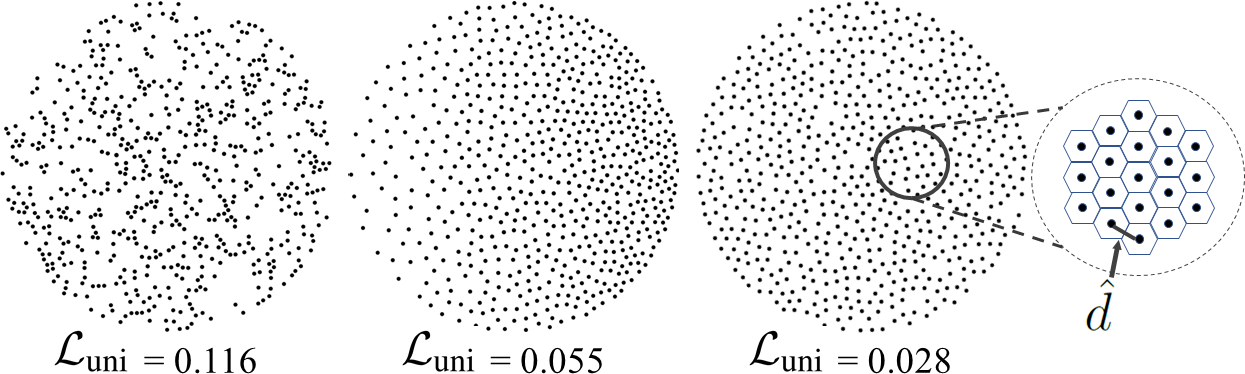
\includegraphics[width=1.0\linewidth]{uniform_example}
	\caption{Example point sets with same number of points (625) but different point distribution patterns; $\mathcal{L_{\text{uni}}}$ is computed with $p$$=$$1\%$.}
%We set $p=1\%$ for uniformity calculation.}
	\label{fig:uniformity}
	\vspace*{-2mm}
\end{figure}

Our method evaluates $\mathcal{Q}$ (a patch of $rN$ points) during the network training by first using the farthest sampling to pick $M$ seed points in $\mathcal{Q}$ and using a ball query of radius $r_d$ to crop a point subset (denoted as $S_j$, $j=1..M$) in $\mathcal{Q}$ at each seed.
Here, we use a small $r_d$, so $S_j$ roughly lies on a small local disk of area $\pi r_d^2$ on the underlying surface.
%
On the other hand, since we form patches by geodesics and normalize them in a unit sphere, patch area is $\sim$$\pi 1^2$.
%generated $\mathcal{Q}$ could be roughly unfolded as a 2D circle with the radius of 1.
%Considering that each training patch $\mathcal{Q}$ is geodesically segmented on the object surface and is normalized within a canonical sphere, each patch thus could be unfolded as a 2D circle with the radius of 1.
So, the expected percentage of points in $S_j$ (denoted as $p$) is $\pi r_d^2 / \pi 1^2 = r_d^2$, and the expected number of points in $S_j$ (denoted as $\hat{n}$) is $rNp$.
%
Hence, we follow the chi-squared model to measure the deviation of $|S_j|$ from $\hat{n}$, and define
%
\begin{equation}
U_{\text{imbalance}}(S_j) = \frac{(|S_j|-\hat{n})^2}{\hat{n}} \ .
\end{equation}

To account for local point clutter, for each point in $S_j$, we find its distance to the nearest neighbor, denoted as $d_{j,k}$ for the $k$-th point in $S_j$.
If $S_j$ has a uniform distribution, the expected point-to-neighbor distance $\hat{d}$ should be roughly $\sqrt{\frac{2\pi r_d^2}{|S_j| \sqrt{3}}}$, which is derived based on the assumption that $S_j$ is flat and neighboring points are hexagonal; see Figure~\ref{fig:uniformity} (right) for an illustration and supplemental material for the derivation.
%
Again, we follow the chi-squared model to measure the deviation of $d_{j,k}$ from $\hat{d}$, and define
%
\begin{equation}
U_{\text{clutter}}(S_j) = \sum_{k=1}^{|S_j|} \frac{(d_{j,k}-\hat{d})^2}{\hat{d}} \ .
\end{equation}
%where $d_{j,k}$ represents the distance between the $k$-th point inside the $j$-th disk and its nearest neighbor.

Here, $U_{\text{clutter}}$ accounts for the local distribution uniformity, while $U_{\text{imbalance}}$ accounts for the nonlocal uniformity to encourage better point coverage.
Putting them together, we formulate the uniform loss as
%
\vspace*{-1.5mm}
\begin{equation}
\label{eq:uniform}
\mathcal{L_{\text{uni}}} = \sum_{j=1}^{M}U_{\text{imbalance}}(S_j) \cdot U_{\text{clutter}}(S_j) \ .
\vspace*{-1mm}
\end{equation}
%
Figure~\ref{fig:uniformity} shows three example point sets with the same number of points but different point distribution patterns.
Using $\mathcal{L_{\text{uni}}}$, we can distinguish the point uniformity among them.
%we can see that, our proposed uniform loss is not only sensitive to local uniformity, but also the global uniformity; see particularly the middle point set.
%


%Then, the area percentage (denoted as $p$) of the local disk over the patch described by $\mathcal{Q}$ can be approximated by $\pi r_d^2/\pi 1^2=r_d^2$.
%with the assumption that the disk is regarded as a 2D circle since it is commonly small enough.
%
%
%We then grow a small disk centered around each seed by using the query ball with the radius of $r_d$.
%Considering that we geodesically \phil{it is wrong to say geodesically here in the training process, right?} crop and normalize each training patch \phil{what exactly is a patch? in methodology, writing should be precise and specific... what is a patch? $\mathcal{Q}$? Never use a term that hasn't been defined clearly in the methodology section}
%within a sphere with radius one, thus the area percentage (denoted as $p$) of the disk over the patch can be calculated \phil{approximated, right?  Another important thing in writing is PRECISION!!!!} by $\pi r_d^2/\pi 1^2=r_d^2$, assuming \phil{..., for small $r_d$.}
%where we approximate both the disk and the patch as 2D circles by considering that the disk is small enough and the patch is geodesically cropped, thus could be unfolded as 2D circles with very few errors.
%\phil{why 1 in the equation? there should be some reasons that you need to explain, right?}
%In our implementation, %instead of a single fixed disk area percentage $p$,
%we obtain multiple small disks around each seed with varying $p$ (\ie, 0.4\%, 0.6\%, 0.8\%, 1.0\%, and 1.2\%).
%For each area percentage $p$, we define $n_j$ as the point number inside the $j$-th disk and $\hat{n}$ as the expected point number for each disk.
%Then, for the $j$-th disk with the number of points as $n_j$, on the one hand,
%If the generated $rN$ points are uniformly-distributed on the patch, the expected point number $\hat{n}$ of each disk can be approximated by $rN \times p$.
%Here, we employ the chi-squared test to measure the imbalance between $n_j$ and $\hat{n}$ given the $j$-th disk, which is denoted as:
%
%\begin{equation}
%	U_{\text{imbalance}}(j) = \frac{(n_j-\hat{n})^2}{\hat{n}}.
%\end{equation}

%On the other hand, if points are uniformly-distributed inside the $j$-th disk of the radius $r_d$ , the expected adjacent point distance $\hat{d}$ can be approximated by $\sqrt{\frac{2\pi r_d^2}{n_j \times \sqrt{3}}}$
%\phil{you MUST prepare a supp. section to derive this number step by step... do it ASAP to make sure that this formulae is correct... I doubt}
%with the assumption that we uniformly split the disk using hexagons of the same size; see the illustration on the rightmost of Figure~\ref{fig:uniformity}.
%Please refer to the supplementary material for the detailed derivation of $\hat{d}$.
%Thus, we formulate the following term to account for the cohesion:
%\begin{equation}
%U_{\text{cohesion}}(j) = \sum_{k=1}^{n_j} \frac{(d_{j,k}-\hat{d})^2}{\hat{d}},
%\end{equation}
%where $d_{j,k}$ represents the distance between the $k$-th point inside the $j$-th disk and its nearest neighbor.

%For the sake of computational efficiency, we design a uniform loss based on a simplified version of the uniformity metric. First, we extract a series of partitions defined as a neighborhood ball in the underlying Euclidean space. To evenly cover the whole surface, the centroids are selected among generated point set by a farthest point sampling (FPS) algorithm. Within our assumption, the normalized patch-based inputs can be regarded as a round surface with a radius 1. Given the size of each neighborhood ball, we can obtain the expected inside number of points $\hat{N}$. In that case, we directly query $\hat{N}$ points for each centroid given a query radius $r$. We will duplicate the centroid point if inside point number is less than $\hat{N}$ and select the nearest $\hat{N}$ point if there are too many point in one ball(whole process is implemented by the ball query ~\cite{qi2017pointnet++}). Finally, the uniform loss is formulated by:

%\begin{equation}
%\mathcal{L_{\text{uni}}} &=& \sum_{D}^{i=0}\sum_{\hat{N}}^{j=0}\left(\frac{(d_{ij}-\hat{d_i})^2}{\hat{d_i}}\right)\\
%\hat{d_i}&=&\sqrt{\frac{2\pi r^2}{\sqrt{3}}}
%\end{equation}
%where $d_{ij}$ represents the distance between $jth$ point and its nearest neighbour and $\hat{d_i}$ is the corresponding expected distance and it will be the same for all balls given a fixed radius.



%%%%%%%%%%%%%%%%%%%%%%%%%%%%%%%%%%%%%%%%%%%%%%

\para{Reconstruction loss.} \
Both the adversarial and uniform losses do not encourage the generated points to lie on the target surface.
Thus, we include a reconstruction loss using the Earth Mover's distance (EMD)~\cite{fan2016point}:
%to emphasize the geometric consistency between the predicted point set and the sampled point set on the surface:
%
\vspace*{-1.5mm}
\begin{equation}
	\mathcal{L_{\text{rec}}} = \min_{\phi:\mathcal{Q}\rightarrow \mathcal{\hat{Q}}} \sum_{q_i\in \mathcal{Q}} \|q_i-\phi(q_i)\|_2,
	\vspace*{-1mm}
\end{equation}
%
where %$\mathcal{\tilde{Q}}$ is a sampled patch of points co-located with $\mathcal{Q}$, simply for representing the underlying object surface, and
$\phi:\mathcal{Q}\rightarrow \mathcal{\hat{Q}}$ is the bijection mapping.



%%%%%%%%%%%%%%%%%%%%%%%%%%%%%%%%%%%%%%%%%%%%%%

\para{Compound loss.} \
Overall, we train PU-GAN end-to-end by minimizing $\mathcal{L}_G$ for generator and  $\mathcal{L}_D$ for discriminator:
\begin{eqnarray}
\label{eq:compound}
	\mathcal{L}_G&=& \lambda_{\text{gan}}\mathcal{L_{\text{gan}}}(G) +\lambda_{\text{rec}}\mathcal{L_{\text{rec}}} + \lambda_{\text{uni}}\mathcal{L_{\text{uni}}}, \\
	\text{and} \ \
    \mathcal{L}_D&=&\mathcal{L}_{\text{gan}}(D),
\end{eqnarray}
where $\lambda_{\text{gan}}$, $\lambda_{\text{rec}}$, and $\lambda_{\text{uni}}$ are weights.
%to balance the relative importance of each loss term.
During the training process, $G$ and $D$ are optimized alternatively.

%why we do not sample centroids on the uniform sample, cause if do so, at the begining, the unform will take a prominent position with a non-uniform outputs, however, we need to be steady to train the nerwork
